\section{Question 3}

\subsection{Question}
Estimate the age of each of the 1000 URIs using the ``Carbon Date'' tool:\\

http://ws-dl.blogspot.com/2013/04/2013-04-19-carbon-dating-web.html\\

Note: you'll have better luck downloading and installing the tool 
rather than using the web service (which will run slowly and likely
be unreliable).\\

For URIs that have > 0 Mementos and an estimated creation date,
create a graph with age (in days) on one axis and number of mementos
on the other.\\

\subsection{Resources}
\begin{itemize}
\item R functions: \url{http://stackoverflow.com/questions/16860200/row-by-row-operations-and-updates-in-data-table}
\item R lapply: \url{http://stackoverflow.com/questions/20766617/using-apply-functions-in-place-of-for-loop-in-r}
\item R strptime: \url{https://stat.ethz.ch/R-manual/R-devel/library/base/html/strptime.html}
\end{itemize}

\subsection{Answer}
Using the python script in Listing \ref{listing:carbondate} to utilize the tools from the 
``Carbon Date'' tool provided by H.S. Eldeen, estimated creation dates were found for
843 of the original URIs. These were stored in the file {\tt site\_ecd\_all}.

\lstinputlisting[language=Python, caption={carbondate.py}, label=listing:carbondate]{q3/carbondate.py}

To prepare the dataset for graphing, the Python script in Listing \ref{listing:bld_ecd} was used to capture the desired subset of data from the {\tt site\_ecd\_all} file; i.e, those site-memento pairs where the memento count was greater than zero. The results were stored in the file {\tt ecd\_mementos}. 

\lstinputlisting[language=Python, caption={build\_ecd\_mementos.py}, label=listing:bld_ecd]{q3/build_ecd_mementos.py}

Using the R script in Listing \ref{listing:graphecd}, with the dataset obtained from Listing \ref{listing:bld_ecd} (the {\tt ecd\_mementos} file), the graph in Figure \ref{fig:ecdgraph} was created. This graph shows that the older a site is the higher that site's memento count tends to be. It also shows that there are a far greater number of new sites than old ones.

\lstinputlisting[language=R, caption={ecd\_mementos\_graph.r}, label=listing:graphecd]{q3/ecd_mementos_graph.r}

\begin{figure}[h!]
\centering
\fbox{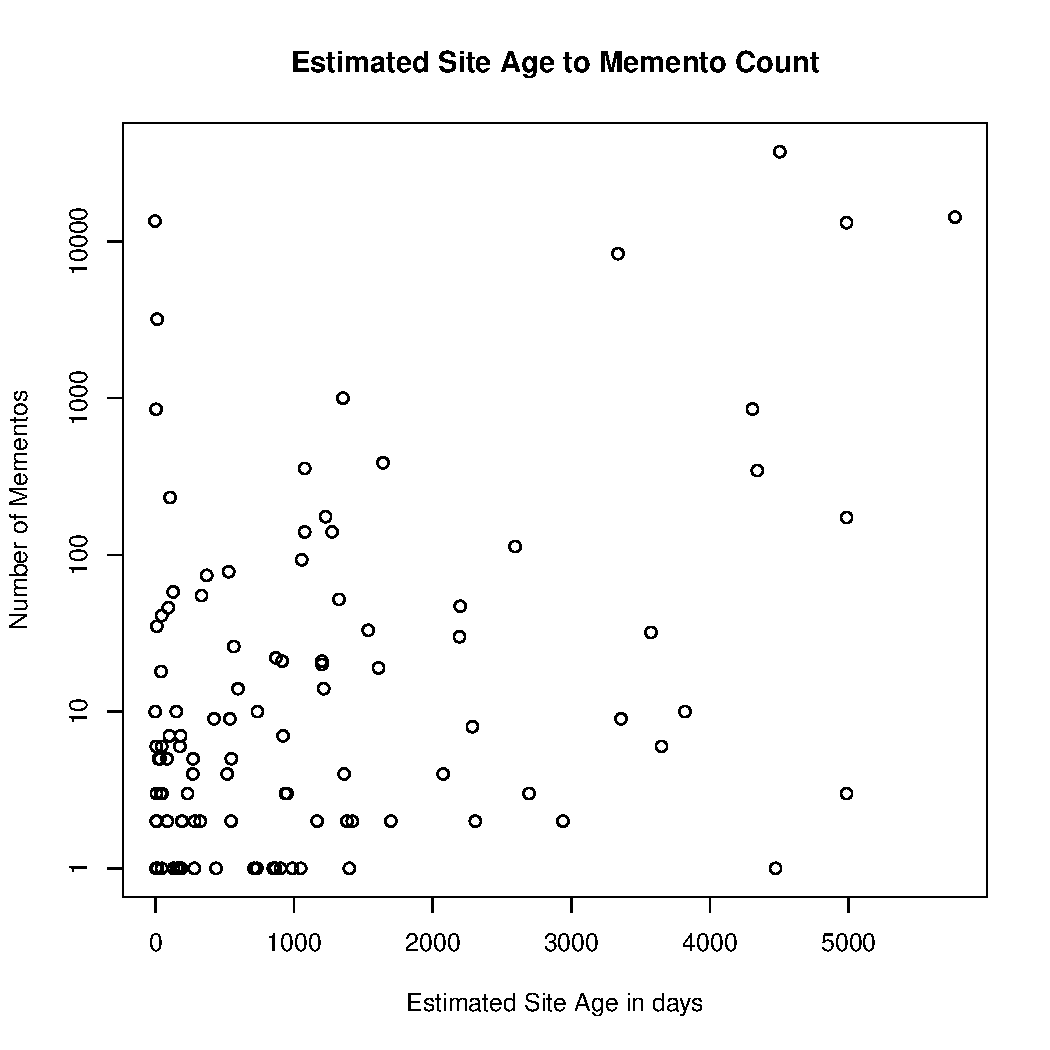
\includegraphics[scale=.65]{q3/ecd_mementos.pdf}}
\caption{Estimated Age to Memento Count}
\label{fig:ecdgraph}
\end{figure}